%% ACM TRUST 2027 submission.
%% Template: acmart v2.21 (2026/11/01), sigconf, as required by the TRUST 2027 author guidelines.
%% Review build: double-blind (anonymous) with line numbers (review).
%% For camera-ready: remove `review,anonymous`, fill in the rights block ACM sends, and restore authors.
\documentclass[sigconf,review,anonymous]{acmart}

%% ---------------------------------------------------------------- packages
\usepackage{booktabs}
\usepackage{multirow}
\usepackage{xspace}
\usepackage{enumitem}
\usepackage{tikz}
\usetikzlibrary{positioning,arrows.meta,fit,calc,shapes.misc}

\setlength{\emergencystretch}{1.5em}

%% ---------------------------------------------------------------- rights block (submission placeholders)
\setcopyright{none}
\settopmatter{printacmref=false}
\renewcommand\footnotetextcopyrightpermission[1]{}
\acmConference[ACM TRUST '27]{ACM Conference on Trustworthy and Responsible AI and Computing Systems}{March 7--9, 2027}{Washington, DC, USA}
\acmYear{2027}
\acmDOI{}
\acmISBN{}

%% ---------------------------------------------------------------- shared macros and result numbers
%% Shared names and terms, so the paper uses one word for each thing.

%% Placeholders for numbers that the main (test) run has not produced yet.
%% Every placeholder renders in red. Before submission, `grep -n "\\tbd\|\\TBD" *.tex sections/*.tex` must be empty.
\newcommand{\tbd}{\textcolor{red}{\textbf{??}}\xspace}
\newcommand{\TBD}[1]{\textcolor{red}{[\textit{#1}]}\xspace}

%% Platforms (systems that build simulator programs)
\newcommand{\otf}{OTF-Tools\xspace}
\newcommand{\devs}{DEVS-Gen\xspace}
\newcommand{\agent}{the plain coding agent\xspace}
\newcommand{\Agent}{The plain coding agent\xspace}

%% Our method and the gate configurations
\newcommand{\gate}{\textsc{Directed}\xspace}
\newcommand{\cfg}[1]{\textsc{#1}\xspace}

%% Decline reasons (plain terms used throughout)
\newcommand{\dterm}[1]{\textsf{#1}}
\newcommand{\Trusted}{\dterm{Trusted}\xspace}
\newcommand{\Caught}{\dterm{Caught}\xspace}
\newcommand{\Already}{\dterm{Already caught}\xspace}
\newcommand{\Untestable}{\dterm{Untestable}\xspace}
\newcommand{\Failhist}{\dterm{Failed history check}\xspace}
\newcommand{\Cantexpress}{\dterm{Can't express}\xspace}
\newcommand{\Badrequest}{\dterm{Request rejected}\xspace}


%% Short forms
\newcommand{\eg}{e.g.,\xspace}
\newcommand{\ie}{i.e.,\xspace}

%% =====================================================================================
%% RESULT NUMBERS QUOTED IN THE PROSE (abstract, introduction, results text, conclusion)
%% =====================================================================================
%% Every value here is a placeholder until the main (test) run is scored by
%% scripts/main_analysis.py. Replace \tbd with the measured value; never with a dev number.
%% Table cells are filled directly in sections/06_results.tex (search for \tbd there).
%%
%% Units: error = wrong answers / answered answers (1 - precision), as a percentage.
%% Coverage = answered program-question pairs / all program-question pairs, as a percentage.
%% "Matched" = the judge is cut to the gate's coverage in each cell (process x builder cohort).
%% The two builder classes (hosted-API models, Ollama models) are never pooled.

%% ---- Hosted-API builder class, all four domains (headline) --------------------------
\newcommand{\rGateCovClaude}{\tbd}        % gate coverage (%)
\newcommand{\rGateErrClaude}{\tbd}        % gate error among answered (%)
\newcommand{\rNoCheckErrClaude}{\tbd}     % error with no added check (native config) (%)
\newcommand{\rHistErrClaude}{\tbd}        % history check only (%)
\newcommand{\rAnsJudgeErrClaude}{\tbd}    % answer-level LLM judge (Haiku) at matched coverage (%)
\newcommand{\rReactErrClaude}{\tbd}       % ReAct judge (Haiku) at matched coverage (%)
\newcommand{\rWrongRemovedClaude}{\tbd}   % share of wrong answers the gate removes (%)
\newcommand{\rRightLostClaude}{\tbd}      % share of correct answers the gate declines (%)

%% ---- Ollama-hosted builder class (OTF-Tools only) -------------------------------------
\newcommand{\rGateCovOllama}{\tbd}
\newcommand{\rGateErrOllama}{\tbd}
\newcommand{\rNoCheckErrOllama}{\tbd}

%% ---- Where the gate's declines come from (Section 6.2) --------------------------------
\newcommand{\rShareCaught}{\tbd}          % share of wrong answers removed that were Caught (%)
\newcommand{\rShareUntestable}{\tbd}      % share of wrong answers removed that were Untestable (%)
\newcommand{\rShareHist}{\tbd}            % share removed by Failed history check (%)

%% ---- Reuse under a changed or reworded policy (Section 6.3) ---------------------------
\newcommand{\rPolPGateErr}{\tbd}
\newcommand{\rPolPHistErr}{\tbd}
\newcommand{\rPolHUnneeded}{\tbd}         % rows rechecked on H that a text-blind record would have carried

%% ---- Cost (Section 6.4) ----------------------------------------------------------------
\newcommand{\rGateExecPerQ}{\tbd}         % program executions per question (median)
\newcommand{\rGateSecPerQ}{\tbd}          % wall-clock seconds per question (median)
\newcommand{\rAnsJudgeUSDPerRow}{\tbd}    % answer-level judge, USD per row (mean)
\newcommand{\rReactUSDPerRow}{\tbd}       % ReAct judge, USD per row (mean)
\newcommand{\rReactSecPerRow}{\tbd}       % ReAct judge, seconds per row (median)
\newcommand{\rTotalUSD}{\tbd}             % all model spend in the study (USD)


\begin{document}

\title{Beyond Pass or Fail: Checking When LLM-Generated Simulators Can Answer What-If Questions}

%% Double-blind: author block is suppressed by `anonymous`. Restore real authors only for camera-ready.
\author{Anonymous Author(s)}
\affiliation{%
  \institution{Anonymous Institution}
  \city{Anonymous City}
  \country{Anonymous Country}}
\email{anonymous@example.com}

\begin{abstract}
%% Registered abstract (2026-11-08, written by the authors), lightly corrected for grammar; the last two sentences
%% report the scored test run (numbers in results.tex).
Large language models can now write simulation programs of operational processes and workflows. These programs can be reused to answer what-if questions on new records and policies. However, a program that reproduces recorded history can still give wrong answers to what-if questions. It may apply the requested change wrongly, apply it to records other than the ones the question is about, or stop being valid once its policy is revised. Current checks return a pass-or-fail verdict for the whole program, which says little about whether any single answer can be trusted. We propose \emph{Vouch}, a library that judges whether an answer from a generated simulator can be trusted for the change being asked about. Each what-if question is turned into a structured change, which is checked against the program and the current records. The library also keeps a record of the kinds of change each program has passed or failed, and repeats the relevant tests whenever the program is reused. We apply it to three program-generation platforms, with programs built by five language models, across four domains: manufacturing, IT operations, and pharmacy and loan application workflows, using independently checked reference answers. Our baselines are the platforms' own checks where such checks exist, an LLM-as-a-judge, and a ReAct agent that can run the program. We measure how many correct answers are trusted, how many are wrongly rejected, how many wrong answers are accepted, and what the checking costs. On programs written by Claude models, \rHistWrongClaude{} wrong answers pass a strict check of recorded history; Vouch lets \rGateWrongClaude{} of them through while still trusting \rGateCovClaude\% of all answers, and at equal coverage it accepts fewer wrong answers than LLM judges built on Claude Haiku. The gain is concentrated on one platform and one kind of change; where the history check already finds the errors, Vouch adds nothing, and after a real change of policy it answers nothing.

\end{abstract}

\ccsdesc[500]{Software and its engineering~Software verification and validation}
\ccsdesc[300]{Computing methodologies~Modeling and simulation}
\ccsdesc[300]{Computing methodologies~Natural language processing}

\keywords{LLM-generated simulators, what-if questions, counterfactual answers, selective answering, assurance, metamorphic testing, process simulation, LLM-as-a-judge}

\maketitle

\section{Introduction}
\label{sec:intro}

Large language models (LLMs) are now capable of writing programs that recompute processes with changes applies to answer what-if questions. that does this recomputing. Given a document that states a process's rules and records its history, a capable model can produce a simulator: code that reads the recorded inputs, applies the rules, and reports what happens~\cite{otftools2026,chen2026devs,holt2025gsim}. Once built, the same program can answer many questions, including ones about new records or a revised policy. Building it once therefore costs far less than having a model reason through the process for each question~\cite{otftools2026}.

This paper studies whether these reusable programs can be trusted. Before a generated program is used, platforms check it. A common check, and a classic test of simulation models~\cite{sargent2013vv}, is whether the program reproduces the recorded history: hide some recorded outcomes, run the program, and compare. We call this a \emph{history check}. A program that passes is accepted and then used for every later question. That verdict is about the program as a whole. A what-if question, however, asks about one particular change, and a program can reproduce history perfectly while handling that change wrongly.

Consider a loan-application process from our benchmark, in which every applicant takes exactly one day to complete a form. During development, a program written by one of our models reproduced every recorded outcome on all four development runs, and the platform's own check accepted it with a perfect score. Reading its code showed why it could not be trusted for every question: it ignored the per-case durations it read from the records and used the published one-day constant instead. Because that duration never varies in the history, no history check can see the problem. Asked ``what if this applicant had finished the form in one second?'', the program answers a full day too late, and the error spreads to other cases that wait for the same workers.

Machine learning has a name for this situation: models that fit the same data equally well can still behave differently on inputs the data never exercised~\cite{damour2022underspecification}. A single pass-or-fail verdict on a program therefore says little about whether a \emph{particular answer}, for a \emph{particular change}, can be trusted. Failures can come from several places: the question may be misread, the change may be applied to the wrong record, the program may ignore the changed input or simulate its effects incorrectly, or the program may stop being valid when the policy it was built for changes. A checker that only judges the program as a whole cannot tell these apart, and cannot tell a user which answers to rely on.

\paragraph{Our approach.} We built Vouch, an assurance library that decides, for each answer, whether to trust it or decline it, based on the change the question asks for. Because the change is an intervention on the process, we call this intervention-level assurance. For each question, Vouch:
\begin{enumerate}[leftmargin=*,nosep]
  \item turns the question into a structured change (what is changed, how, by how much, when, and for which record) and checks that change against the document and the current records;
  \item checks that the program reproduces the recorded history of the run being asked about;
  \item runs small tests aimed at the requested \emph{kind} of change, built only from the document's stated rules and records, never from reference answers; for example, it changes the same kind of input for another case and checks that the program's output moves, and that nothing before the change moves;
  \item keeps a record of which kinds of change each program has passed or failed, so that a failure blocks later answers that depend on the same kind of change, and repeats the relevant tests when the program is reused on new records or under a new policy.
\end{enumerate}
Every decline comes with a reason in plain terms: a test showed the program getting this kind of change wrong (\Caught), it had failed the same test on an earlier question (\Already), no test of this kind of change could run on the program (\Untestable), the program does not reproduce the recorded history (\Failhist), or it has no input that can represent the change (\Cantexpress).

\paragraph{Evaluation.} We evaluate Vouch as one of several \emph{trust judges}, procedures that decide whether to trust an answer, all deciding about the same fixed programs, questions and answers. The other judges are each platform's own acceptance check, the history check by itself, generic tests that are not aimed at the requested change, agreement with an answer an LLM gives by reading the document, an LLM asked to judge the answer, an LLM asked to judge the program, and a ReAct agent~\cite{yao2023react} that can run the program in a sandbox before deciding. Programs come from three platforms (\otf~\cite{otftools2026}, \devs~\cite{chen2026devs}, and a plain coding agent), built by five LLMs, in four domains: manufacturing, IT operations, and loan and pharmacy workflows. Reference answers come from separately implemented and independently checked reference simulators, never from an LLM. Because a judge can always look safer by answering less, we compare judges at the \emph{same answer coverage}, and we report the cost of each.

\paragraph{Findings.} With no added check, \rNoCheckWrongClaude{} of the answers given by programs that Claude models wrote are wrong (\rNoCheckErrClaude\%). The history check leaves \rHistWrongClaude{} of them, and Vouch leaves \rGateWrongClaude{} while trusting \rGateCovClaude\% of all questions. Almost all of the difference comes from one platform, where \rOtfHistWrong{} wrong answers pass the history check and Vouch trusts none of them, at the cost of 123 of the 2{,}052 correct answers the history check keeps. Every one of these wrong answers came from a correctly interpreted question, so the faults lie in the programs. Where the history check already finds the errors, or programs make none, Vouch adds nothing. At equal coverage it accepts fewer wrong answers than LLM judges built on Claude Haiku, and ties with stronger and open-weight judges that we ran on small samples. When the rules change, here by adding one worker to a pool, every program fails the history check and Vouch answers nothing, while agreement with a reading answer keeps nearly half of the answers without error. Vouch needs no extra model calls and about \rGateExecPerQ{} extra program runs per question.

\paragraph{Contributions.}
\begin{itemize}[leftmargin=*,nosep]
  \item Vouch, a method for deciding whether to release a generated simulator's answer to a what-if question: it checks the structured request against the records, tests the requested kind of change without reference answers, consults the failures recorded for the program, and names the reason for every decline (\S\ref{sec:method}).
  \item A benchmark and protocol for answer-level assurance: 547 test questions in four domains with exact answers under fixed random draws, independently checked reference answers, no-effect controls and policy variants, and 86 programs from three platforms and five builder models, judged with the candidate answers held fixed (\S\ref{sec:problem}, \S\ref{sec:benchmark}, \S\ref{sec:judges}).
  \item An account of when answer-level checking helps and when it does not, against rule-based and LLM judges at equal coverage, reported per platform, domain, kind of change and program (\S\ref{sec:results}).
\end{itemize}

\section{Problem Setting}
\label{sec:problem}

\paragraph{Documents, runs and programs.} A \emph{document} describes one process. Its front matter states the rules: the steps, which workers or machines do them, working hours, how cases are routed, how capacity is shared. The rest of the document holds one or more \emph{runs}. Each run records the inputs (arrivals, planned work, orders, task requests) and the outcomes (when each case ended, what shipped, when each task started). A \emph{platform} reads a development document and produces a \emph{program}: a simulator that takes a run's inputs and returns its outcomes. The same program is later applied to other runs of the same process, which it has never seen.

\paragraph{Questions.} A what-if question names a run, one \emph{change} to it, and one queried outcome. For example: ``In Run~11, suppose 1 Technician worker (Technician\_7) was unavailable from time 28800 to time 43200. At what time would case c0014 end?'' Each change belongs to a \emph{family}, a kind of change such as a different activity duration, a different routing probability, or fewer workers (Table~\ref{tab:benchmark}). Some valid changes do not affect the queried outcome. These \emph{no-effect controls} are included on purpose: a judge that distrusts every answer that ``did not move'' is wrong on them.

\paragraph{Answers.} To answer, the platform applies the change to the run's inputs, runs the program, and reads off the queried value. An answer is \emph{correct} if it equals the reference answer (numbers within one unit). A program may also produce no answer, for instance when it has no input that can represent the change.

\paragraph{Trust judges.} A \emph{trust judge} sees a program, a run, a question and, depending on the judge, the program's answer, and decides to \emph{trust} or \emph{decline}. All judges decide about the same programs and the same answers, so they differ only in which answers they let through. We count an answer as \emph{answered} only if it is trusted \emph{and} the program produced it; a trusted row with no answer counts as declined. This rule is the same for every judge.

\paragraph{What we measure.} The unit is one program--question pair. For each judge, within one process and one cohort of programs (same platform and builder model):
\begin{itemize}[leftmargin=*,nosep]
  \item \textbf{coverage}: answered pairs as a share of all pairs;
  \item \textbf{error}: wrong answers as a share of answered pairs (one minus precision), and the count of wrong answers accepted;
  \item \textbf{correct kept}: correct answered pairs as a share of all pairs, and \textbf{correct declined}: correct program answers that the judge declined;
  \item \textbf{cost}: program executions, model calls, tokens, dollars and wall-clock time spent on judging.
\end{itemize}
A judge that answers less can always look safer. We therefore compare judges at \emph{matched coverage}: judges that give a confidence are cut at the coverage our library reaches in the same cell, keeping their most confident answers, with ties resolved by their exact expected precision. Judges that give only a yes or no are reported at their own operating point, next to a random refusal at the library's coverage. Programs built by different model families are never pooled.

\section{The Assurance Library}
\label{sec:method}

\begin{figure*}[t]
\centering
%% Figure 1: the decision pipeline (TikZ, full text width, left to right).
\resizebox{\textwidth}{!}{%
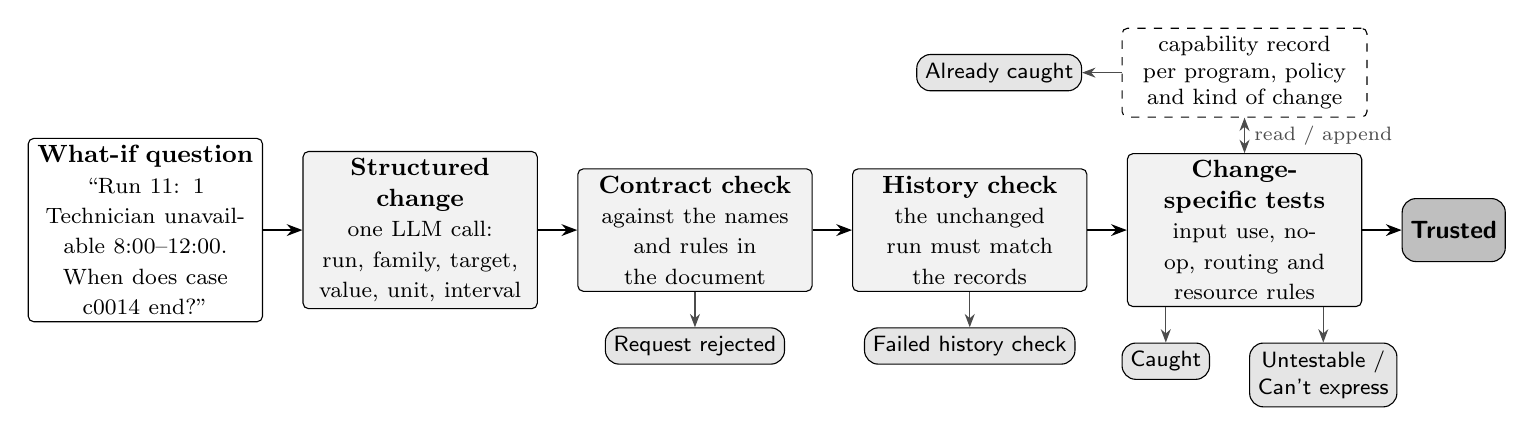
\begin{tikzpicture}[
  font=\small,
  node distance=4.5mm and 5mm,
  pStage/.style={draw, rounded corners=2pt, fill=black!5, align=center, text width=2.8cm, minimum height=13mm, inner sep=2.5pt},
  pIO/.style={draw, rounded corners=2pt, fill=white, align=center, text width=2.8cm, minimum height=13mm, inner sep=2.5pt},
  pOut/.style={draw, rounded corners=5pt, align=center, inner sep=3pt, fill=black!10, font=\footnotesize\sffamily},
  pRec/.style={draw, dashed, rounded corners=2pt, align=center, inner sep=3pt, font=\footnotesize, text width=2.9cm},
  pArr/.style={-{Stealth[length=2mm]}, semithick},
  pSide/.style={-{Stealth[length=1.7mm]}, thin, black!70}
]
\node[pIO]    (q) {\textbf{What-if question}\\\footnotesize ``Run 11: 1 Technician unavailable 8:00--12:00. When does case c0014 end?''};
\node[pStage, right=of q] (i) {\textbf{Structured change}\\\footnotesize one LLM call: run, family, target, value, unit, interval};
\node[pStage, right=of i] (c) {\textbf{Contract check}\\\footnotesize against the names and rules in the document};
\node[pStage, right=of c] (h) {\textbf{History check}\\\footnotesize the unchanged run must match the records};
\node[pStage, right=of h] (p) {\textbf{Change-specific tests}\\\footnotesize input use, no-op, routing and resource rules};
\node[pOut, right=of p, fill=black!25, minimum height=8mm, font=\small\sffamily\bfseries] (t) {Trusted};

\node[pOut, below=of c] (o1) {Request rejected};
\node[pOut, below=of h] (o2) {Failed history check};
\node[pOut, below=of p, xshift=-10mm] (o3) {Caught};
\node[pOut, below=of p, xshift=10mm] (o4) {Untestable /\\Can't express};
\node[pRec, above=of p] (r) {capability record per program, policy and kind of change};
\node[pOut, left=of r] (o5) {Already caught};

\draw[pArr] (q) -- (i);
\draw[pArr] (i) -- (c);
\draw[pArr] (c) -- (h);
\draw[pArr] (h) -- (p);
\draw[pArr] (p) -- (t);
\draw[pSide] (c) -- (o1);
\draw[pSide] (h) -- (o2);
\draw[pSide] (p.south -| o3) -- (o3.north);
\draw[pSide] (p.south -| o4) -- (o4.north);
\draw[pSide, {Stealth[length=1.7mm]}-{Stealth[length=1.7mm]}] (r) -- node[right, font=\scriptsize]{read / append} (p);
\draw[pSide] (r) -- (o5);
\end{tikzpicture}}

\caption{How the library decides about one what-if answer. Each check can decline, and each decline is named for what the library observed. Tests use only the document and runs of the program, never reference answers. The capability record carries test results between questions and is consulted again when the program is reused.}
\Description{A top-to-bottom flow. A what-if question is interpreted into a structured change, which passes a contract check, a history check, and change-specific tests that read and write a capability record. Passing all steps gives Trusted. Side exits are labelled Request rejected, Failed history check, Caught, Already caught, Untestable, and Can't express.}
\label{fig:pipeline}
\end{figure*}

The library decides, for one question and one program, whether the program's answer can be trusted. It is a Python package of about 3.8k lines that platforms call through a small adapter: the adapter runs the program on a given set of inputs and returns its output records. Figure~\ref{fig:pipeline} shows the steps. The configuration that runs all of them is called \gate. Every step uses only what a user of the platform could legitimately see: the document and runs of the program on inputs the library constructs. No step reads a reference simulator, a reference answer, or any hidden label.

\subsection{From question to a checked change}
\label{sec:method:request}

One LLM call (Claude Haiku~5.5) turns the question into a structured change: the run, the family, the operation (for example \emph{set}, \emph{add workers}, \emph{remove}), the selected case and target (an activity, a wait, a decision point, a worker pool, a product, a task), the visit, the new value with its unit, the effective time interval, and the queried outcome. This output is not trusted. A \emph{contract check} compares it with a description of the process built from the document alone: the names of runs, cases, activities, pools and decision points, and the stated routes and pool sizes. It separates an unknown target, an ambiguous match, an unsupported operation, an invalid unit, an invalid time interval, a non-numeric value and an unreadable question. Any of these declines the request before the program is run (\Badrequest). Removing the very case being asked about, for example, is rejected as an unsupported operation.

\otf answers through its own path, in which another LLM call edits the program's extracted records to apply the change~\cite{otftools2026}. For these programs the library also compares the records before and after the edit. A case-level change must alter exactly one input record, for the requested case and target, to the requested value, and must change nothing else. A failed comparison declines the answer even if the answer happens to be right, so a wrong edit is never rewarded.

\subsection{History check}
\label{sec:method:history}

The program is run on the unchanged inputs of the run being asked about, and its outcomes must equal the recorded ones exactly (every case end in a workflow; every ledger cell in manufacturing; every task-log event in IT). This is stricter than \otf's acceptance check, which compares predicted with hidden events under a time tolerance and accepts a mean F1 of~0.4~\cite{otftools2026}. A program that fails is declined on that run (\Failhist). The history check alone is also one of the judges we compare against.

\subsection{Tests aimed at the requested change}
\label{sec:method:probes}

A history check cannot see a mistake in an input that never varied, as in the example of \S\ref{sec:intro}. The library therefore changes inputs itself and checks properties that any correct simulator must satisfy. Each test states its expected relation, and each relation follows from the document's rules and records rather than from a reference answer. In software-testing terms they are metamorphic relations~\cite{chen2018metamorphic,segura2016survey}. Tests are chosen by the requested family and target:
\begin{itemize}[leftmargin=*,nosep]
  \item \textbf{Input use.} Change the same kind of input for \emph{another} case that the records show was used (one hour more work or delay, or a route draw that selects a different stated route). That case's outputs must change, and no output earlier than the point where the changed input is first used may change. A crash fails the test. This is the test that exposes the program in \S\ref{sec:intro}.
  \item \textbf{No-op.} Change an input for a visit that the records show never happened. Nothing may change.
  \item \textbf{Routing rule.} When route probabilities change, the printed draws decide which recorded decisions switch route. The earliest switched decision must take its new route and nothing before it may move; if no decision switches, the outputs must not change at all.
  \item \textbf{Resource rules.} A worker made unavailable starts no task inside the interval. With added workers, nothing changes before the first task of that pool that had to wait, and that task starts earlier.
  \item \textbf{Case removal.} Remove a different case: its records must vanish, and nothing before its arrival may move.
  \item \textbf{Exact stated-rule checks.} Where a program prints records that name tasks, waits, workers and visits, the library recomputes what the stated rules imply for a test change (task and wait timing, case paths implied by the printed draws, which workers can be used) and compares. Manufacturing and IT have analogous checks for dispatch completeness and for resource requests.
\end{itemize}
A test that cannot be run (no suitable second case, or no input that can represent the change) counts neither as a pass nor as a failure. \gate trusts an answer only if at least one test that exercises the changed input ran and passed, and none failed. A passing no-op alone never suffices. Main tests are capped at three program executions per request; the stated-rule checks add their own executions, which we count.

\subsection{A record of what each program can do}
\label{sec:method:registry}

Every test result is appended to a \emph{capability record}, keyed by the program's code hash, the adapter version, a fingerprint of the stated policy, the family and the operation. A record has one of three states: \emph{failed}, \emph{untested}, or \emph{tested under the listed conditions}; it never says ``verified''. Reuse follows two rules. First, a failure blocks the capability for that target wherever the key matches, so a program caught once is not trusted on the same kind of change later (\Already). Second, a pass is reused only for the same key on the same run; on new records or under a changed policy, the relevant tests are run again. Passes that depend on the request's own values, such as new route probabilities or a particular unavailability interval, are never reused. The policy fingerprint hashes the front matter without the list of runs, so new runs under the same rules keep the same fingerprint, while any change to the rule text, including a harmless rewording, forces rechecking. We measure the cost of that choice in \S\ref{sec:results:reuse}.

\subsection{Decisions in plain terms}
\label{sec:method:terms}

Each decline is named for what the library saw. \Caught: a test showed the program getting this kind of change wrong. \Already: it failed this test on an earlier question. \Untestable: no test of this kind of change could run on this program, so the library has no evidence either way. \Failhist: the program does not reproduce the recorded history of this run. \Cantexpress: the program has no input that can represent the change. \Badrequest: the structured change failed the contract check. Otherwise the answer is \Trusted. These names separate declines that \emph{detect} a problem (\Caught, \Already, \Failhist) from declines that only \emph{abstain} (\Untestable, \Cantexpress), which matters when reading the results.

\paragraph{Ablations.} The same code path gives simpler configurations: \cfg{Schema} (contract check only), \cfg{Replay} (contract and history check), \cfg{Generic} (contract, history and input-use tests on randomly chosen families, with the same execution budget as \gate), and \cfg{Program-wide} (one verdict per program and run from one input-use test per case-level family, the same for every question on that run).

\paragraph{Running untrusted code.} Generated programs run inside a sandbox (bubblewrap with every namespace unshared, only system libraries and the program's own folder mounted, no network, and a seccomp filter that allows only local sockets). Reference code and gold are outside the sandbox.

\section{Benchmark}
\label{sec:benchmark}

\begin{table*}[t]
\centering
\caption{Domains, change families and test questions. Every family has valid no-effect controls. Inputs are real for manufacturing and IT and come from published process models for the workflows; all outcomes are computed under the rules stated in each document.}
\label{tab:benchmark}
\small
\begin{tabular}{@{}l p{4.6cm} p{6.6cm} r r@{}}
\toprule
Domain & Source of inputs and rules & Change families (what a question changes) & Test qs. & No-effect \\
\midrule
Loan application & Published BPMN model and simulation parameters~\cite{chapela2023zenodo}; 17 activities, loops, 6 worker pools & activity duration; timer delay; route draw of one case; routing probabilities; worker availability (added or unavailable workers); case removal & 120 & 24 \\
Pharmacy & Same source; 12 activities, loops, 3 worker pools & same six families & 120 & 24 \\
Manufacturing & SupplyGraph production and orders~\cite{wasi2024supplygraph}; written dispatch policy~\cite{otftools2026} & order removal; production quantity; production timing; dispatch capacity & 96 & 16 \\
IT operations & Google 2011 cluster trace~\cite{reiss2011google}; written priority scheduler on 8 machines~\cite{otftools2026} & job removal; machine-failure removal; task priority; task resource request; machine removal & 120 & 20 \\
\midrule
Policy reuse (workflows) & Loan and Pharmacy under a changed policy (P: one more worker in one pool) or a reworded one (H: same rules, 24 sentences rewritten) & the six workflow families & 91 & 22 \\
\bottomrule
\end{tabular}
\end{table*}

\paragraph{Domains.} Table~\ref{tab:benchmark} lists the four domains. The two workflows come from an open collection of business-process models with simulation parameters~\cite{chapela2023zenodo,chapela2024extraneous}. We chose Loan Application and Pharmacy because they have distinct structures, queues, loops and timer events. Manufacturing and IT operations reuse the documents of a prior process-record benchmark~\cite{otftools2026}: real production, order and cluster-trace inputs, with outcomes computed under a written dispatch policy and a written scheduler. Each workflow run has 15 cases; a manufacturing run is one plant over 14 days; an IT run is one cluster window.

\paragraph{Exact answers to what-if questions.} A what-if question has an exact answer only if the random parts of a run are pinned down. A shared random seed does not do this: in the Prosimos simulator~\cite{lopezpintado2023prosimos}, for example, draws come from process-wide streams in execution order, so adding one case changed the routes of earlier cases in our checks. We therefore wrote the workflow semantics down first (resource allocation, calendars, priorities, simultaneous events, timers, routing and loops) and built a deterministic reference engine for it. Every random quantity is tied to a stable identity (case, activity or decision, visit) and printed in the document: planned work, planned waits, and route draws to six decimals. Removing a case leaves every other case's draws unchanged, and a new routing probability is applied to the same draw. This is a common-random-numbers coupling~\cite{law2015simulation}: the question asks about the same realized run under a change, and everything needed for the exact answer is in the document. Manufacturing and IT are deterministic by construction.

\paragraph{Checked reference answers.} Gold never comes from an LLM judge. For the workflows, an independent checker was written from the semantics specification alone, without the engine's code or outputs. Engine and checker agree on 18 of 18 hand-worked cases, on 66 of 66 fixed scenarios and 500 of 500 randomized ones in every output field, and on all 240 workflow test questions. A further check confirms that every value each test answer depends on is printed in the document (240 of 240), and that rounding the printed route draws changes no answer. Separately started agents, given only the document text, reproduced every printed record of the sampled runs and matched gold on 24 of 24 sampled questions. For manufacturing and IT, gold comes from the original simulators and from a second implementation fed only by values parsed back from the documents; the two agree on all 216 test questions, and blind samples matched on 16 of 16 (manufacturing, by hand) and 20 of 20 (IT, agents writing their own schedulers). Prosimos was used only to compare factual aggregates, which cannot validate what-if answers.

\paragraph{Questions and splits.} Test questions are drawn by a fixed rule, never by how any system performs on them. Each family has 20 (workflow) or 24 (manufacturing, IT) test questions, of which one in five or one in six is a no-effect control. Rules applied at generation remove questions whose answer needs an unprinted draw, changes equal to the recorded value, changes at visits that never happen (an unknown target, not a no-effect change), and unavailability of workers who do no work. Splits are by run: development runs 1--4 and test runs 5--12 for each workflow, with policy-variant runs 13--16. IT windows that share jobs and manufacturing periods that share order-book days are kept on the same side. The development set (112 workflow, 108 manufacturing and IT questions) was used to design the library; it is not reported as evidence.

\paragraph{Policy reuse.} The policy set (Table~\ref{tab:benchmark}, last row) tests reuse when the rules themselves move. In variant P one pool gets one more worker (Loan Appraisers 2$\to$3; Pharmacy Pharmacists 1$\to$2), stated in the document. In variant H the parameters are byte-identical and 24 sentences of the rules are reworded; four blind agents reproduced every H run from the H text, confirming the rules did not change. A program that hard-codes the old pool size should fail on P. A judge that treats any text change as a new policy will recheck H needlessly.

\begin{table}[t]
\centering
\caption{Programs evaluated, as accepted builds out of build attempts. All were built on development documents only and reused on unseen test runs. B0 is the original \otf code, kept unchanged and used only with its own check.}
\label{tab:programs}
\small
\setlength{\tabcolsep}{3.2pt}
\begin{tabular}{@{}ll rrrr r@{}}
\toprule
Platform & Builder & Loan & Pharm. & Mfg. & IT & Accepted \\
\midrule
\otf (R1) & Sonnet 5.5 & 3 & 3 & 3 & 3 & 12/12 \\
          & Haiku 5.5  & 3 & 3 & 3 & 3 & 12/12 \\
          & gpt-oss-120b & 2 & 3 & 3 & 2 & 10/12 \\
          & Gemma 4 31B  & 3 & 2 & 3 & 3 & 11/12 \\
          & Qwen3.5 9B   & 2 & 0 & 0 & 1 & 3/12 \\
\otf (B0) & Sonnet 5.5 & 3 & 3 & 3 & 3 & 12/12 \\
          & Haiku 5.5  & 3 & 3 & 2 & 2 & 10/12 \\
          & gpt-oss-120b & 2 & 2 & 1 & 3 & 8/12 \\
          & Gemma 4 31B  & 0 & 1 & 0 & 1 & 2/12 \\
          & Qwen3.5 9B   & 0 & 0 & 0 & 0 & 0/12 \\
\devs     & Sonnet 5.5 & 3 & 3 & 3 & 3 & 12/12 \\
          & Haiku 5.5  & 2 & 3 & 3 & 2 & 10/13 \\
Coding agent & Sonnet 5.5 & 2 & 2 & 2 & 2 & 8/8 \\
          & Haiku 5.5  & 2 & 2 & 2 & 2 & 8/8 \\
\midrule
\multicolumn{2}{@{}l}{Total} & 30 & 30 & 28 & 30 & 118/161 \\
\bottomrule
\end{tabular}
\end{table}

\paragraph{Platforms and programs.} Three platforms build programs (Table~\ref{tab:programs}). \textbf{\otf}~\cite{otftools2026} compiles a document into reader functions and a simulator, accepts a program if it reproduces hidden recorded outcomes well enough, and answers by having an LLM edit the extracted records and re-running the simulator. We use its original code unchanged as \textbf{B0}, and a generation path we call \textbf{R1} that fixes mechanical failures we diagnosed in B0 builds (a helper that makes record locations correct by construction, more reading attempts, and failure feedback that leads with the fix); R1 gives no hints about process logic and keeps the acceptance check unchanged. \textbf{\devs}~\cite{chen2026devs} generates discrete-event models in stages from a specification; we give it the document's rules and one generic input format for records, plans and probabilities. \textbf{\Agent} is a single model asked to write a simulator for the same specification and run it once on a published example input, without further checks. Programs are built by Claude Sonnet~5.5 and Haiku~5.5 on every platform, and by gpt-oss-120b~\cite{openai2025gptoss}, Gemma~4 31B and Qwen3.5~9B through Ollama on \otf only. Builds are independent, none was selected by result, and failed builds are reported. While building, builders had no access to test documents, gold or reference code; we checked this with sandbox isolation tests and by scanning every program for test-only names, seeds and draws.

In total, the main test set has 9{,}792 program--question pairs from the 86 programs that are judged (2{,}640 Loan, 2{,}520 Pharmacy, 2{,}112 manufacturing, 2{,}520 IT), and the policy set has 1{,}411 pairs from the 31 Claude-built workflow programs. B0's 32 programs add pairs that are scored only under their own check.

\section{Trust Judges Compared}
\label{sec:judges}

The benchmark yields 9{,}792 program--question pairs, each with a fixed answer or none, and every judge decides about each of them. All judges receive the same structured change (\S\ref{sec:method:request}), so differences come from how they judge, not from how the question was read. No judge sees reference answers, reference simulators, the hidden correct reading of the question, other programs, other judges' verdicts or build histories.

\paragraph{Rule-based judges.} Four judges run on every pair without model calls. The \emph{platform check} trusts every answer from an accepted program; it is the single verdict a platform gives today, and for the coding agent it means only that the program ran. The \emph{history check} trusts an answer if the program reproduces the queried run exactly. \emph{Generic tests} add input-use tests on randomly chosen families to the history check, with Vouch's budget of program runs. \emph{Disagreement} trusts an answer if it agrees with a \emph{reading answer}, which Claude Haiku gives after reading the rules and the queried run, without any program.

\paragraph{LLM judges.} Each LLM judge returns a verdict, a confidence from 0 to 100 that the answer is exactly right, and a one-line reason; a reply that cannot be parsed, is cut off, is refused or runs out of turns counts as a decline. The \emph{answer-level judge}~\cite{zheng2023judging} makes one call that sees the rules, the queried run's records, the program's code, the question, the structured change, the answer and the unchanged answer. The \emph{program-level judge} makes one call per program and run, without the question and answer, and its verdict covers every question on that run. The \emph{ReAct judge}~\cite{yao2023react} alternates reasoning with actions; its one tool runs Python in a sandbox holding the program and the same document view, for at most eight turns. It is told what to return and nothing about how to test, and since it can run the program on any input, it has at least Vouch's access to execution. The three form a ladder from reasoning alone, to reasoning with free execution, to Vouch's fixed tests. The answer-level and ReAct judges also see the question text and the answer, which Vouch never uses.
%% D30 (Jev answer-level judge): add here and to Table 3 only once its run is scored.

\paragraph{Models and subsets.} Interpretation and reading answers use Claude Haiku~5.5 for every platform. LLM judging is costly, so it ran on fixed subsets of answered pairs, drawn by pair identifier with a fixed seed before any judging, balanced across domain, platform, builder model and family, and taken from the main and policy sets together. The Haiku answer-level judge saw 3{,}000 pairs, the Haiku ReAct judge 1{,}000 of them, and the Haiku program-level judge every program and run. A shared subset of 150 pairs was judged by all five models with the answer-level judge and by Haiku, gpt-oss, Gemma and Qwen with the ReAct judge; Sonnet's ReAct judge saw 50 of those. We report each judge on the Claude-built main-test pairs of its subset (for example, 2{,}028 of the 3{,}000). Because LLM judges see only pairs that have an answer, their coverage is a share of answered pairs and so higher than coverage over all pairs. Two reduced versions of Vouch, the contract check alone and program-wide tests, and a random refusal at Vouch's coverage complete the comparison.

\paragraph{Analysis plan.} Vouch, the runner, the scorer, the judge prompts, the questions, the splits and the program list were frozen and hashed before any test question was run. Later changes were raised spending limits, the open-weight and Sonnet ReAct judges added on the shared subset, subsets drawn from the policy set as well, the run-level analysis described below, and a rerun without the capability record (\S\ref{sec:results:families}); no code, prompt or program changed, and every change is logged. Uncertainty comes from a two-level bootstrap with 2{,}000 resamples of programs and then questions, with the coverage match redone in every resample and every difference computed on the same resamples. Because questions on one run share records and draws, we repeated the analysis resampling whole runs, and call a difference significant only if its 95\% interval excludes zero under both versions.

\section{Results}
\label{sec:results}

%% NOTE FOR FILLING IN: every \tbd and \TBD below is a placeholder for a number or finding from the
%% scored test run (scripts/main_analysis.py on wf_test, ml_test, wf_policy and runs/judges_main_v1).
%% Do not fill any cell from development data. Prose marked \TBD states what the sentence must report;
%% rewrite it to match the measured direction, including null or negative results.

We ask four questions. \textbf{RQ1}: at the same coverage, does the library accept fewer wrong answers than the other judges? \textbf{RQ2}: when it declines, is it detecting errors or abstaining? \textbf{RQ3}: does rechecking keep wrong answers out when a program is reused under a changed policy, and what does it cost when the policy was only reworded? \textbf{RQ4}: what does checking cost? All numbers are from the test runs, with programs built on development documents only.

\subsection{RQ1: Wrong answers accepted at matched coverage}
\label{sec:results:main}

\begin{table*}[t]
\centering
\caption{Coverage (Cov.) and error among answered pairs (Err., \%) on the test runs. Claude-built programs pool \otf R1, \devs and the coding agent within each domain as sums over cells; Ollama-built programs (\otf R1 only) are shown apart. LLM judges are cut to \gate's coverage in each cell (matched); rule-based judges are shown at their own operating point. 95\% two-level bootstrap intervals are in the artifact.}
\label{tab:main}
\small
\setlength{\tabcolsep}{4.2pt}
\begin{tabular}{@{}l rr rr rr rr rr@{}}
\toprule
& \multicolumn{8}{c}{Claude-built programs} & \multicolumn{2}{c}{Ollama-built (\otf)} \\
\cmidrule(lr){2-9}\cmidrule(l){10-11}
& \multicolumn{2}{c}{Loan} & \multicolumn{2}{c}{Pharmacy} & \multicolumn{2}{c}{Manufacturing} & \multicolumn{2}{c}{IT operations} & \multicolumn{2}{c}{All domains} \\
Judge & Cov. & Err. & Cov. & Err. & Cov. & Err. & Cov. & Err. & Cov. & Err. \\
\midrule
Platform check (no added check) & \tbd & \tbd & \tbd & \tbd & \tbd & \tbd & \tbd & \tbd & \tbd & \tbd \\
History check (\cfg{Replay}) & \tbd & \tbd & \tbd & \tbd & \tbd & \tbd & \tbd & \tbd & \tbd & \tbd \\
Generic tests (\cfg{Generic}) & \tbd & \tbd & \tbd & \tbd & \tbd & \tbd & \tbd & \tbd & \tbd & \tbd \\
Disagreement with reading & \tbd & \tbd & \tbd & \tbd & \tbd & \tbd & \tbd & \tbd & \tbd & \tbd \\
Program-level LLM judge (Haiku) & \tbd & \tbd & \tbd & \tbd & \tbd & \tbd & \tbd & \tbd & \tbd & \tbd \\
\midrule
Answer-level LLM judge (Haiku), matched & \tbd & \tbd & \tbd & \tbd & \tbd & \tbd & \tbd & \tbd & \tbd & \tbd \\
ReAct judge (Haiku), matched & \tbd & \tbd & \tbd & \tbd & \tbd & \tbd & \tbd & \tbd & \tbd & \tbd \\
Random refusal, matched & \tbd & \tbd & \tbd & \tbd & \tbd & \tbd & \tbd & \tbd & \tbd & \tbd \\
\midrule
\cfg{Schema} (ablation) & \tbd & \tbd & \tbd & \tbd & \tbd & \tbd & \tbd & \tbd & \tbd & \tbd \\
\cfg{Program-wide} (ablation) & \tbd & \tbd & \tbd & \tbd & \tbd & \tbd & \tbd & \tbd & \tbd & \tbd \\
\gate (ours) & \tbd & \tbd & \tbd & \tbd & \tbd & \tbd & \tbd & \tbd & \tbd & \tbd \\
\bottomrule
\end{tabular}
\end{table*}

Table~\ref{tab:main} gives the main comparison. Without any added check, \TBD{\rNoCheckErrClaude\% of answers from Claude-built programs are wrong; state per domain where errors concentrate}. The history check \TBD{removes X of these at a coverage cost of Y; report \rHistErrClaude\%}. \gate reaches \rGateCovClaude\% coverage with \rGateErrClaude\% error, removing \rWrongRemovedClaude\% of the wrong answers and declining \rRightLostClaude\% of the correct ones. At the same coverage, the answer-level LLM judge has \rAnsJudgeErrClaude\% error and the ReAct judge \rReactErrClaude\%. \TBD{State the paired difference and interval for gate minus each judge, and say plainly where the gate is not better.}

\TBD{Domain by domain. Report separately (i) domains where programs make few or no errors, so that any judge can only lose coverage there; (ii) the IT result, where a capability caught once blocks that family for the program everywhere, and the coverage this costs on otherwise correct answers; (iii) whether \cfg{Generic} with the same budget recovers the gate's gain, which tells whether the choice of test matters.}

For Ollama-built programs, \TBD{report \rNoCheckErrOllama\% vs.\ \rGateErrOllama\% at \rGateCovOllama\% coverage; most of these programs fail the history check, so state how much of the difference is the history check alone}. Qwen built only three programs, so its cells are thin evidence.

\paragraph{Per program.} \TBD{One sentence per platform on spread across individual programs (from the per-program table in the artifact): how many programs have any wrong answer trusted by the gate, and whether one program dominates the totals.}

\subsection{RQ2: Detecting or abstaining?}
\label{sec:results:families}

\begin{table}[t]
\centering
\caption{The gate's decisions by change family (Claude-built programs, test). ``Wrong'' is the number of wrong answers with no added check; ``Kept'' the wrong answers the gate trusts. Declines are split into those that \emph{detect} (\Caught, \Already, \Failhist) and those that \emph{abstain} (\Untestable, \Cantexpress, \Badrequest), each as wrong answers removed / correct answers lost.}
\label{tab:families}
\footnotesize
\setlength{\tabcolsep}{3pt}
\begin{tabular}{@{}l r r r c c@{}}
\toprule
Family & Pairs & Wrong & Kept & Detect & Abstain \\
\midrule
\multicolumn{6}{@{}l}{\textit{Workflows (Loan and Pharmacy)}} \\
Activity duration & \tbd & \tbd & \tbd & \tbd/\tbd & \tbd/\tbd \\
Timer delay & \tbd & \tbd & \tbd & \tbd/\tbd & \tbd/\tbd \\
Route draw (one case) & \tbd & \tbd & \tbd & \tbd/\tbd & \tbd/\tbd \\
Routing probabilities & \tbd & \tbd & \tbd & \tbd/\tbd & \tbd/\tbd \\
Worker availability & \tbd & \tbd & \tbd & \tbd/\tbd & \tbd/\tbd \\
Case removal & \tbd & \tbd & \tbd & \tbd/\tbd & \tbd/\tbd \\
\multicolumn{6}{@{}l}{\textit{Manufacturing}} \\
Order removal & \tbd & \tbd & \tbd & \tbd/\tbd & \tbd/\tbd \\
Production quantity & \tbd & \tbd & \tbd & \tbd/\tbd & \tbd/\tbd \\
Production timing & \tbd & \tbd & \tbd & \tbd/\tbd & \tbd/\tbd \\
Dispatch capacity & \tbd & \tbd & \tbd & \tbd/\tbd & \tbd/\tbd \\
\multicolumn{6}{@{}l}{\textit{IT operations}} \\
Job removal & \tbd & \tbd & \tbd & \tbd/\tbd & \tbd/\tbd \\
Failure removal & \tbd & \tbd & \tbd & \tbd/\tbd & \tbd/\tbd \\
Task priority & \tbd & \tbd & \tbd & \tbd/\tbd & \tbd/\tbd \\
Task resource request & \tbd & \tbd & \tbd & \tbd/\tbd & \tbd/\tbd \\
Machine removal & \tbd & \tbd & \tbd & \tbd/\tbd & \tbd/\tbd \\
\midrule
No-effect controls (all) & \tbd & \tbd & \tbd & \tbd/\tbd & \tbd/\tbd \\
\bottomrule
\end{tabular}
\end{table}

A judge can remove wrong answers in two ways: by finding the error, or by declining questions it cannot check. Both reduce accepted errors, but only the first is evidence about the program. Table~\ref{tab:families} separates them. Of the wrong answers \gate removes, \rShareCaught\% are \Caught or \Already, \rShareHist\% fail the history check, and \rShareUntestable\% are declined as \Untestable. \TBD{Name the families where the gain is mainly abstention, and where the tests detect errors the history check cannot see, with one concrete example of a \Caught program (what the test changed and what moved).} On no-effect controls, \TBD{report whether any correct ``nothing changes'' answer was declined, and why}.

\paragraph{Interpretation.} \TBD{Share of test questions whose structured change matched the hidden binding exactly, per domain; and how the gate's error and coverage change when the hidden binding is supplied instead (oracle request), which bounds the share of errors due to misreading the question.}

\subsection{RQ3: Reuse under a changed or reworded policy}
\label{sec:results:reuse}

\begin{table}[t]
\centering
\caption{Policy reuse (Claude-built workflow programs; 1{,}411 pairs). Programs and their capability records come from the test runs. P changes one pool size; H rewords the rules without changing them. Exec./pair counts program executions per question.}
\label{tab:reuse}
\footnotesize
\setlength{\tabcolsep}{3pt}
\begin{tabular}{@{}l rr rr r@{}}
\toprule
& \multicolumn{2}{c}{P (changed)} & \multicolumn{2}{c}{H (reworded)} & \\
\cmidrule(lr){2-3}\cmidrule(lr){4-5}
Judge (recheck regime) & Cov. & Err. & Cov. & Err. & Exec./pair \\
\midrule
Platform check (no recheck) & \tbd & \tbd & \tbd & \tbd & 0 \\
History check (factual recheck) & \tbd & \tbd & \tbd & \tbd & \tbd \\
\gate (per-family recheck) & \tbd & \tbd & \tbd & \tbd & \tbd \\
\bottomrule
\end{tabular}
\end{table}

Every main result above is already a reuse result: each program was built on development runs and judged on test runs it had never seen, and its capability record carried failures from earlier test questions forward. Table~\ref{tab:reuse} adds a change of the rules themselves. Under P, \TBD{report how many programs keep the old pool size, whether the history check exposes them, and the gate's error \rPolPGateErr\% vs.\ \rPolPHistErr\% for the history check}. No P decision used evidence recorded under the old policy (\TBD{confirm the count is 0}). Under H, the fingerprint treats the rewording as a new policy, so the gate rechecks everything: \TBD{report the extra executions, and the number of rows (\rPolHUnneeded) where a failure recorded on test was dropped although the rules had not changed, and how many of those answers were wrong}. This is the price of a text-level fingerprint, and we report it rather than tune it away.

\subsection{RQ4: Cost of checking}
\label{sec:results:cost}

\begin{table}[t]
\centering
\caption{Cost per judged pair on the test runs. Program executions exclude the run that produces the answer. USD at list prices.}
\label{tab:cost}
\footnotesize
\setlength{\tabcolsep}{3pt}
\begin{tabular}{@{}l r r r r@{}}
\toprule
Judge & Model calls & USD & Executions & Seconds \\
\midrule
History check & 0 & 0 & \tbd & \tbd \\
Generic tests & 0 & 0 & \tbd & \tbd \\
\gate & 0 & 0 & \tbd & \tbd \\
Answer-level judge, Haiku & 1 & \tbd & 0 & \tbd \\
Answer-level judge, Sonnet & 1 & \tbd & 0 & \tbd \\
Program-level judge, Haiku$^\dagger$ & \tbd & \tbd & 0 & \tbd \\
ReAct judge, Haiku & \tbd & \tbd & \tbd & \tbd \\
ReAct judge, Sonnet & \tbd & \tbd & \tbd & \tbd \\
\bottomrule
\multicolumn{5}{@{}l}{\scriptsize $^\dagger$One call per program and run, spread over its questions.}\\
\multicolumn{5}{@{}l}{\scriptsize The shared interpretation call (Haiku) is not counted here; every judge uses it.}
\end{tabular}
\end{table}

The library's checks make no model calls beyond the shared interpretation; their cost is program executions. \gate uses a median of \rGateExecPerQ executions and \rGateSecPerQ seconds per question (Table~\ref{tab:cost}). The answer-level judge costs \$\rAnsJudgeUSDPerRow per pair and the ReAct judge \$\rReactUSDPerRow and \rReactSecPerRow seconds. \TBD{State how cost scales with reuse: passing evidence is reused within a run, so the per-question cost falls when many questions share a run; give the measured reuse share.}

\subsection{Do LLM judges depend on the model?}
\label{sec:results:models}

\begin{table}[t]
\centering
\caption{The shared 150-pair subset: error at the gate's coverage on these pairs, and the share of replies that could not be parsed (counted as declines). Sonnet ReAct ran on 50 of the 150.}
\label{tab:models}
\footnotesize
\setlength{\tabcolsep}{3.5pt}
\begin{tabular}{@{}l rr rr@{}}
\toprule
& \multicolumn{2}{c}{Answer-level judge} & \multicolumn{2}{c}{ReAct judge} \\
\cmidrule(lr){2-3}\cmidrule(l){4-5}
Model & Err. & Unparsed & Err. & Unparsed \\
\midrule
Claude Haiku 5.5 & \tbd & \tbd & \tbd & \tbd \\
Claude Sonnet 5.5 & \tbd & \tbd & \tbd & \tbd \\
gpt-oss-120b & \tbd & \tbd & \tbd & \tbd \\
Gemma 4 31B & \tbd & \tbd & \tbd & \tbd \\
Qwen3.5 9B & \tbd & \tbd & \tbd & \tbd \\
\midrule
\gate on the same pairs & \multicolumn{4}{c}{\tbd} \\
\bottomrule
\end{tabular}
\end{table}

Table~\ref{tab:models} asks whether a stronger or different model makes a better judge on the same pairs. \TBD{Report the ordering and whether any model's judge beats the gate at matched coverage. Note self-judging: Claude and Ollama models judge programs built by their own family.} In development checks, gpt-oss under our plain-text ReAct format often described an action without writing code; we ran it unchanged, so its ReAct numbers measure that setup with that model, not the model's ability to test programs.

\section{Related Work}
\label{sec:related}

\paragraph{LLM-generated simulators.} Several systems build executable models from text. \otf compiles process-record documents into reusable readers and simulators and accepts a program if it reproduces hidden recorded outcomes~\cite{otftools2026}. \devs generates discrete-event models from specifications and validates their event traces against temporal, causal and semantic constraints derived from the specification~\cite{chen2026devs}. G-Sim proposes simulator structure with an LLM and calibrates parameters against data~\cite{holt2025gsim}. Program-aided reasoning more generally lets a model write code and trusts its execution~\cite{gao2023pal}. Closest in spirit, a validation-aware framework for LLM-driven simulation separates whether a simulation runs from whether its numbers are valid~\cite{yoo2026validation}, and work on LLM agents as suppliers of Modelica models asks what an acceptance test actually certifies~\cite{frochte2026modelica}. These systems judge a model, a run or a trace. We ask a narrower question that arises once a model is reused: whether one answer, for one requested change, can be trusted, and we keep evidence per kind of change across reuse.

\paragraph{Structured requests and abstention.} Turning a natural-language what-if request into a checkable specification has been used to build interactive what-if interfaces, where many generated specifications are wrong even when they compile~\cite{gathani2026praxa}. For database answers consumed as fact, a deterministic kernel that answers only a bounded set of question shapes, and abstains otherwise, keeps a generative front end from choosing the returned value~\cite{wu2026never}. Our contract check plays a similar role for changes, but the decision to trust rests on tests of the program. Selective prediction studies the trade-off between coverage and risk~\cite{elyaniv2010selective,geifman2017selective}, and conformal risk control has been extended to agent trajectories~\cite{opoku2026toolchain}. We borrow the coverage-matched comparison, but our gate is binary, makes no calibration assumption, and claims no guarantee.

\paragraph{Models as judges.} LLMs are widely used to grade other models' outputs~\cite{zheng2023judging}, and they can favor outputs from their own family~\cite{panickssery2024self}, which matters here because the same model families build and judge programs. ReAct interleaves reasoning with tool calls~\cite{yao2023react}; our ReAct judge gives it a code tool and the program. Choosing between text reasoning and program execution per question has also been studied as model selection~\cite{zhao2023selection}. Agreement between independent answerers is a common reliability signal, but errors they share stay invisible to it~\cite{zerhoudi2026wrong}; we include disagreement with a reading answer as a judge for that reason.

\paragraph{Testing simulation programs.} Comparing a model's output with recorded history is a standard validation technique for simulation models~\cite{sargent2013vv}. Our change-specific tests are metamorphic relations~\cite{chen2018metamorphic,segura2016survey}: properties that must hold between runs on related inputs when no oracle for the output exists. One of our IT checks, which removes the dominating machine so that a resource-request test can tell CPU from memory, follows constraint-based test-data generation~\cite{demillo1991constraint}. Fixing exogenous draws so that a factual and a changed run can be compared exactly is the common-random-numbers idea from simulation~\cite{law2015simulation}, and matches the structural view of counterfactuals in which exogenous variables are held fixed~\cite{pearl2009causality}. Process mining and business-process simulation supply the workflow models we use~\cite{vanderaalst2016process,lopezpintado2023prosimos,chapela2024extraneous}.

\section{Limitations}
\label{sec:limits}

\paragraph{The reference and the builders share a model family.} Claude models helped write the workflow semantics, the reference engine and the hand-worked cases, a separately started Claude model wrote the independent checker, and Claude models built and judged programs. A misreading of the semantics shared by the reference and the Claude-built programs would be invisible to our scoring; independent reproductions from the document text reduce this risk but do not exclude it.

\paragraph{Scope.} The workflow runs are fixed realizations of two published synthetic models, with every random draw printed, which real operations would not know in advance. Questions come from templates and are easier to interpret than questions written by people. Finally, \Trusted means only that specific tests passed.

\section{Conclusion}
\label{sec:conclusion}

A generated simulator that reproduces history earns a pass, but a what-if question asks about one change, and the pass does not say whether that change is handled correctly. We built a library that decides per answer: it checks the requested change against the records, checks the program's history on the queried run, tests the requested kind of change with reference-free metamorphic tests, and keeps a per-program record of what was tested, rechecked on reuse. Across four domains, three platforms and five builder models, and against platform checks, history replay, generic tests, disagreement, LLM judges and a ReAct judge at matched coverage, \TBD{one-sentence summary of the measured outcome, including where the library did not help}. The decline reasons make the difference between detecting an error and abstaining visible, which we think a trustworthy answering system should report. Remaining blind spots, a reference written by the same model family as some builders, and a policy fingerprint that rechecks harmless rewordings are the main things to address next.

\paragraph{Artifact.} An anonymized artifact with the library, adapters, benchmark generators, question files with hashes, frozen program lists, judge prompts, all raw decision rows and the analysis scripts is provided for review. \TBD{Insert the anonymous artifact link.} The workflow models are released under CC BY 4.0~\cite{chapela2023zenodo}.


%% Exempt from the page limit (TRUST 2027 author guidelines): GenAI Usage Disclosure and references.
\section*{GenAI Usage Disclosure}
%% Required by ACM TRUST 2027; exempt from the page limit.

Generative AI was used in this work in three ways, which we separate.

\paragraph{As objects of study.} Claude Sonnet~5.5, Claude Haiku~5.5, gpt-oss-120b, Gemma~4 31B and Qwen3.5~9B built the simulator programs we evaluate. Claude Haiku~5.5 interpreted every question, produced the reading answers, and performed \otf's record edits. These five models also served as the LLM-based judges described in \S\ref{sec:judges}. All model calls, tokens, costs and failures are logged in the artifact.

%% AUTHORS: confirm this paragraph matches how the software was actually written before submission.
\paragraph{In building the research software and the benchmark.} An AI coding assistant (Claude, through Claude Code) wrote most of the code of the assurance library, the adapters, the reference engine for the workflows, the question generators, the runners and the analysis scripts, under the authors' direction and review. Claude models also wrote the workflow semantics specification and the hand-worked validation cases, and a separately started Claude model wrote the independent checker from the specification alone. Separately started AI agents performed blind sampled checks of gold answers and independent code reviews of the library, the scorer and the sandbox. Because the same model family wrote the reference and built some of the programs, we treat shared misreadings as a threat to validity (\S\ref{sec:limits}). Every design decision, freeze and post-freeze change was made or approved by the authors and is recorded in a decision log in the artifact.

\paragraph{In writing this paper.} An AI assistant (Claude) drafted the text of this manuscript from the project's design records and results files, under the authors' direction. The authors reviewed and revised the text and are responsible for all claims. All reported numbers come from the scored runs, not from the assistant, and every citation was checked against its DOI, arXiv record or publisher page.


\bibliographystyle{ACM-Reference-Format}
\bibliography{references}

\end{document}
